% !TEX encoding = UTF-8 Unicode
\documentclass[10pt, a4paper]{article}

\usepackage{amsmath}
\usepackage{footnote}
\makesavenoteenv{tabular}
\usepackage{ltc05}
%\usepackage{polski}
\usepackage[utf8]{inputenc}
\usepackage{textcomp} 
\usepackage[T1]{fontenc}
\usepackage{lmodern}
\usepackage{url}
\usepackage{graphicx}
\title{A Sequential Child-Combination Tree-LSTM Network for Sentiment Analysis}


%%%%%%%%%%%%%%%%%%%%%%%%%%%%%%%%%%%%%%%%%%%%%%%%%%%%%%%%%%%%%%%%%%%%%%%%%
%!!!!!!!!!!!!!!!!!!!!!!!!!!!!!!!!!!!!!!!!!!!!!!!!!!!!!!!!!!!!!!!!!!!!!!!!
%!!!!!!!!!!!!!!!!!!!!!!!!!!!!!!!!!!!!!!!!!!!!!!!!!!!!!!!!!!!!!!!!!!!!!!!!
% PLEASE DO NOT WRITE YOUR NAME AND ADDRESS IN THE DRAFT OF YOUR PAPER
% SIMPLY ERASE THE LINES...
\name{Michał Lew$^{\dagger}$\\ \bf \large Piotr Pęzik$^{\ast}$} 

\address{ $^{\dagger}$VoiceLab \\	
               michal.lew@voicelab.pl \\ \\
               $^{\ast}$University of Lodz \\ 
               piotr.pezik@uni.lodz.pl}

%% ... UP TO HERE
% ... UP TO HERE
%!!!!!!!!!!!!!!!!!!!!!!!!!!!!!!!!!!!!!!!!!!!!!!!!!!!!!!!!!!!!!!!!!!!!!!!!
%!!!!!!!!!!!!!!!!!!!!!!!!!!!!!!!!!!!!!!!!!!!!!!!!!!!!!!!!!!!!!!!!!!!!!!!!
%%%%%%%%%%%%%%%%%%%%%%%%%%%%%%%%%%%%%%%%%%%%%%%%%%%%%%%%%%%%%%%%%%%%%%%%%


\abstract{This paper describes a sentiment analysis system based on tree-structured long short-term memory (LSTM) neural networks. As a potential improvement over currently used approaches, we propose a sequential mechanism of combining network units representing syntactic phrases, which provides an alternative way of preserving the compositionality of syntactic parents as combinations of their dependents. We train and evaluate our system on a dataset provided in the PolEval 2017 competition. Our best result obtained with the proposed approach outperforms both basic, linearly combined LSTMs and as well as a related tree-structured variant of such networks.}

\begin{document}

\maketitleabstract

\section{Introduction}   
Sentiment Analysis (SA) is an active area of natural language processing research with applications in product and political marketing, customer relations management systems and social media communication studies to mention just a few examples. A common objective of SA is to automatically detect the attitudinal value of an utterance or otherwise coherent stretch of text which can be attributed to a particular author. The distribution of  such attitudinal values in an utterance is usually known as its \textit{polarity} and it usually ranges from positive to neutral and negative \cite{cambria_schuller}, possibly with finer-grained distinctions between these main categories, such as \textit{somewhat positive} or \textit{very negative} \cite{socher2013recursive}. More recent approaches to SA focus on phrase-level polarity classification, whereby attitudinal or emotional values are detected at the level of syntactic phrases and only then compositionally combined to compute the polarity of an entire utterance. Such approaches are particularly important in aspect-based SA, where different aspects of one's opinion about a product, movie, person, etc. have to be detected in addition to  classifying the overall sentiment of a text unit. Also, phrase-level models of SA are better suited to deal with basic syntactic phenomena such as negation or modality, which may cause a significant shift in the predominant sentiment of an utterance \cite{wilson_wiebe}. 
\par The present paper evaluates a deep-learning based system for syntax-driven SA, which was submitted to the PolEval 2017 competition. We first briefly describe the PolEval sentiment treebank (a syntactically annotated sentiment dataset) and the nature of the classification task. Next, we present the Sequential Child-Combination Tree-LSTM Network model of the proposed system and evaluate its performance on the PolEval test set.


\section{PolEval 2017}

The dataset released in the PolEval competition for the task described in this paper can be described as a sentiment dependency treebank. In general, sentiment treebanks are collections of syntactically parsed sentences which have sentiment annotations assigned to their constituent words or phrases. The type of sub-sentential word combinations which are annotated with  sentiment labels may depend on the exact syntactic formalism used in a given treebank. For example, the Stanford Sentiment Treebank \cite{socher2013recursive} contains full constituency parse trees comprising phrases associated with five sentiment classes. On the other hand, the sentences provided in the PolEval dataset, are dependency-parsed. As we explain below, this distinction has some implications for modeling an SA system which makes use of syntactic annotations. For example, unlike the above-mentioned constituency representations, most sentence dependency graphs are N-ary trees of arbitrary length in that a word node may directly govern only one or more than two other word vertices as in the sentence shown in Fig. \ref{fig:dep_sent}, where the verb \textit{drażni} has four direct dependents (if we count the punctuation mark as a dependent of the sentence root), and the noun \textit{dniu} has only one dependent adjective \textit{całym}. 
\par This example sentence\footnote{Its word-for-word into English could be \textit{(It) doesn't irritate even after a whole day.}} also illustrates the point of using syntactic annotation in sentiment analysis. It is quite evident that it expresses a customer's overall satisfaction with a particular brand of perfume, even though its (directly negated) main verb \textit{drażnić} (irritate) could be found in a list of keywords which generally denote a negative sentiment. On a more subtle level, the positive attitude of this utterance towards this particular product is further reinforced by the indirectly negated adverbial clause (i.e. \textit{even after a whole day}), which denotes a typical condition in which other fragrances might become irritating.
\par Table \ref{tab:nie_drazni_1} illustrates the type of annotations made available in the PolEval 2017 sentiment analysis datasets. For each word in a sentence (listed in row \texttt{W}) its parent word node was indicated (see row \texttt{P}) together with its sentiment label (as in row \texttt{S}). The parent labels could be used to reconstruct the syntactic dependency tree of this sentence as shown in Fig. \ref{fig:dep_sent}. The goal of the PoleVal SA subtask was to  a) correctly identify sentiment labels of each leaf word node and b) to correctly predict the sentiment label of every complete subtree starting in every non-terminal node of the sentence tree. The list of such leaf nodes and subtrees for which sentiment labels would have to be detected if the example sentence was found in the test set is shown in Table \ref{tab:nie_drazni_2}. The overall sentiment of an utterance is thus predicted from the sentiment value of its root node, which is usually the main verb of a sentence and the subtrees of the dependency trees considered in this task (other than the terminal word nodes) are self-contained phrases. 
\begin{table}[h]
 \begin{center}
\begin{tabular}{|l| l l l l l l l|}
      \hline
      %Level&Tools\\
      %\hline\hline
      W & Nie & drażni & nawet & po & całym & dniu & . \\
      \hline
      P & 2 & 0 & 2 & 2 & 6 & 4 & 2 \\
      \hline
      S & 0 & 1 & 0 & 0 & 0 & 0 & 0 \\
      \hline
\end{tabular}
\caption{An example PolEval dataset sentence with phrase-level sentiment annotation (W -- word nodes, P -- syntactic parents, S -- polarity value).}
\label{tab:nie_drazni_1}
 \end{center}
\end{table}



\begin{figure}
  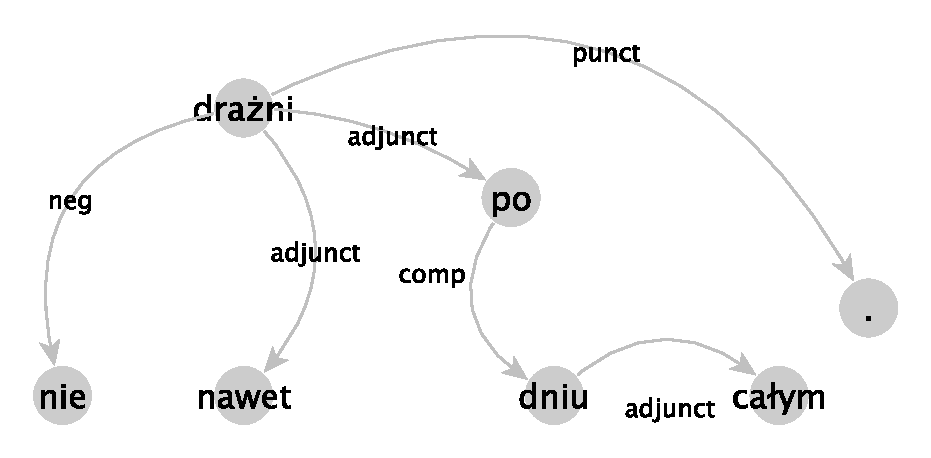
\includegraphics[width=\linewidth]{imgs/nie_drazni.pdf}
  \caption{A dependency representation of the example sentence shown in Table \ref{tab:nie_drazni_1}.}
  \label{fig:dep_sent}
\end{figure}

\begin{table}[h]
 \begin{center}
\begin{tabular}{|l | l|}

\hline
 Word &	Polarity\\
      \hline \hline
     Nie &	0\\
     \hline
Nie drażni nawet po całym dniu	 . & 1\\
\hline
nawet &	0\\
\hline
po całym dniu &	0\\
\hline
całym dniu &	0\\
\hline
.	& 0\\
      \hline
\end{tabular}
\caption{Phrase- and word-level sentiment values to be predicted for the example sentence shown in Table \ref{tab:nie_drazni_1}.}
\label{tab:nie_drazni_2}
 \end{center}
\end{table}

\section{The Model} 


\subsection{LSTM Neural Networks}

Different variants of Recurrent Neural Networks (RNNs) have been widely used for many tasks in natural language processing such named entity recognition \cite{lample2016neural} or text classification \cite{lai2015recurrent}. RNNs can process arbitrarily long inputs by recurrent application of a transition function over hidden states. The most common form of an RNN transition function is an affine transformation followed by a hyperbolic tangent function:
	\begin{equation} h_t = tanh(W_{x_t}+U_{h_{t-1}}+b)
\end{equation}
	A potential advantage of RNNs in processing natural language stems from their ability to use information gathered sequentially from previous states, corresponding to units of language such as words or phrases when dealing with current input. In theory this makes them capable of tracking a long history of previous states when processing sequences of words. In practice, however, RNNs may they suffer from the so-called vanishing gradient problem, which means that during training the gradient can grow or decay exponentially over long sequences \cite{bengio1994learning,hochreiter1998vanishing}. The LSTM architecture \cite{hochreiter1997long} addresses the problem of learning long-term dependencies by introducing a memory cell that is capable of preserving previous state information over relatively long sequences of states.
\par While there are many different types of LSTMs, in our work we used a variant described by the following equations:
		
\begin{equation}
\begin{split}
		&i_t = \sigma(U^i{x_t} + W^is_{t-1} + b^i) ,\\
		&f_t = \sigma(U^f{x_t} + W^fs_{t-1} + b^f) ,\\
		&o_t = \sigma(U^o{x_t} + W^os_{t-1} + b^o) ,\\
		&g_t = \tanh(U^g{x_t}+ W^gs_{t-1} + b^g) ,\\
		&c_t = c_{t-1} \bullet f_t + g_t \bullet i_t ,\\
		&s_t = \tanh(c_t) \bullet o_t 
\end{split}
\end{equation}

		where $x_t$ is input at current time step, $i_t$ is an input gate, $f_t$ a forget gate, $o_t$ an output gate and $c$ stands for LSTM memory.
		The gating mechanism controls how much information from past states and memory is used at the current time step. 

\subsection{Tree LSTMs}
\begin{figure}[h]
	\begin{center}
		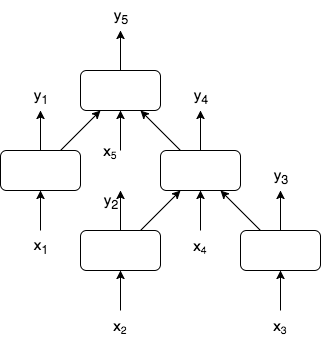
\includegraphics[width=0.3\textwidth]{imgs/tree-lstm}
		\caption{A Tree LSTM network architecture.}
		\label{tab:tree-lstm}
	\end{center}
\end{figure}
	One problem with applying classical LSTMs in natural language processing is that similarly to standard RNNs, they are linear chains, which makes them difficult to use directly for processing more sophisticated linguistic structures. For example, syntactic annotation which could be useful in predicting more subtle aspects of sentiment of the kind illustrated above usually takes the form of hierarchically-structured dependency or constituency trees rather then linear sequences of word segments. In order to process tree-structured data, the standard LSTM architecture has been elaborated into the so-called Tree LSTMs \cite{tai2015improved}.
	In general, Tree-Structured Recurrent Neural Networks expand basic RNNs by creating a way to plug in more than one previous state to a hidden unit at given time step as shown in Figure 2. Each neural network unit takes an input $x_j$ and emits a label $y_j$ as in a standard RNN. Additionally, each such unit can take more than one previous hidden state. Tree-LSTMs also add their memory-handling capacities to this elaborated architecture.
	
\subsection{Tree LSTM label classification}

As already mentioned, in sentiment treebanks, sentences are represented as trees whose (selected) components are also labelled for sentiment. Generally, in a Tree LSTM network used for language processing tasks which can be described as label classification, each sentence component is a unit $x_j$ represented by a distributional vector known as its \textit{(word) embedding} \cite{mikolov2013distributed}. The hidden states of network units which represent the leaves of a syntactic sentence tree are embeddings of the corresponding words. Network units which represent non-terminal tree nodes, have hidden states representing the embeddings of the entire subtree which they have. By computing an activation function on such hidden states, we obtain a sentiment label of an entire subtree. The hidden state of the root unit is the embedding of the entire sentence and its label is the label of the entire sentence.
\par	Tree LSTM architectures may vary with respect to the exact way in which the child units are incorporated into their respective parents. In this paper we consider the so-called Child-Sum Tree-LSTM architecture \cite{tai2015improved} and present a new architecture, which we call a Sequential Child-Combination Tree-LSTM and evaluate its performance in syntax-based sentiment analysis. The Child-Sum Tree-LSTM model (ibid.) provides a way of representing dependency syntax relations between parent word nodes and their children and it is based on the following transitions equations:
\begin{equation}
\begin{split}
&s_{ch}=\sum_{k}s_{ch_k},\\
&i_j = \sigma(U^ix_j + W^is_{ch} + b^i) ,\\
&f_{jk} = \sigma(U^fx_j + W^fs_{ch_k} + b^f) ,\\
&o_j = \sigma(U^ox_j + W^os_{ch} + b^o) ,\\
&g_j = \tanh(U^gx_j+ W^gs_{ch} + b^g) ,\\
&c_j = \sum_{k} c_k \bullet f_{jk} + g_{j} \bullet i_{j} ,\\
&s_j = \tanh({c_{j}}) \bullet o_{j},\\
\end{split}
\end{equation}
	where $k$ is a subscript of $k$-th child of node $j$ and $s_{ch_k}$ is its hidden state. There is no theoretical limit on the branching factor of the syntactic trees to be represented in this architecture. Moreover, as hypothesized by its authors, this model may be capable of learning parameters \textit{W\textsuperscript{i}} which `open' the input gate \textit{$i_{j}$} for semantically discriminative content words such as adjectives or verbs and `close' it for low-information function word inputs such as determiners. 
\subsection{Sequential-Child-Combination Tree-LSTM}

\begin{figure}[h]
	 \begin{center}
    	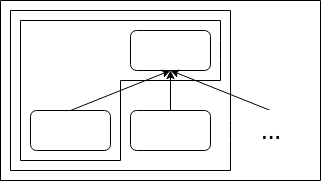
\includegraphics[width=0.3\textwidth]{imgs/sequentialchild}
		\caption{Sequentially combining children with their parents in an LSTM network.}
		\label{tab:sequentialchild}
	 \end{center}
\end{figure}
	The key contribution to LSTM-based models for sentiment analysis proposed in the present paper is what we call a Sequential Child-Combination Tree-LSTM architecture. Formally, in order to combine, children nodes with their parents, we follow the transition equations specified below:
\begin{equation}
\begin{split}
&i_{i_1} = \sigma(U^i{x_t} + W^i{s_{ch_1}} + b^i) ,\\
&f_{i_1} = \sigma(U^f{x_t} + W^f{s_{ch_1}} + b^f) ,\\
&o_{i_1} = \sigma(U^o{x_t} + W^o{s_{ch_1}} + b^o) ,\\
&g_{i_1} = \tanh(U^g{x_t}+ W^g{s_{ch_1}} + b^g) ,\\
&c_{i_1} = c_{t-1} \bullet f_{i_1} + g_{i_1} \bullet i_{i_1} ,\\
&s_{i_1} = \tanh({c_{i_1}}) \bullet o_{i_1},\\\\
&i_{i_2} = \sigma(U^is_{i_1} + W^is_{ch_2} + b^i) ,\\
&f_{i_2} = \sigma(U^fs_{i_1} + W^fs_{ch_2} + b^f) ,\\
&o_{i_2} = \sigma(U^os_{i_1} + W^os_{ch_2} + b^o) ,\\
&g_{i_2} = \tanh(U^gs_{i_1}+ W^gs_{ch_1} + b^g) ,\\
&c_{i_2} = c_{i_1} \bullet f_{i_2} + g_{i_2} \bullet i_{i_2} ,\\
&s_{i_2} = \tanh(c_{i_2}) \bullet o_{i_2},\\\\
&\cdots\\\\
&i_{i_n} = \sigma(U^is_{{n-1}} + W^is_{ch_{n}} + b^i) ,\\
&f_{i_n} = \sigma(U^fs_{{n-1}} + W^fs_{ch_{n}} + b^f) ,\\
&o_{i_n} = \sigma(U^os_{{n-1}} + W^os_{ch_{n}} + b^o) ,\\
&g_{i_n} = \tanh(U^gs_{{n-1}}+ W^gs_{ch_{n}} + b^g) ,\\
&c_{i_n} = c_{i_{n-1}} \bullet f_{i_n} + g_{i_n} \bullet i_{i_n} ,\\
&s_{i_n} = \tanh(c_{i_n}) \bullet o_{i_n},\\\\
&c_{t} = c_{i_n}\\
&s_{j} = s_{i_n}
\end{split}
\end{equation}
	where $s_{i_k}$ is an intermediate state obtained after combining with its $k$-th child. That means that we can see each Tree-LSTM unit as a linear LSTM chain representing each child respectively with $c$ as one global, linearly updated memory.
\par Even though dependency trees do not explicitly encode word order information, the proposed method of combining them allows for creating embeddings composed of subphrases or single word dependents of particular children and `remember' them in the learning process, which is not directly possible in case of the Child-Sum Tree-LSTM architecture. Moreover, word order information can be preserved in our model by combining first the children that occur earlier in the sentence. The intuition behind this approach is to provide a mechanism of encoding  the relations between the parent and its particular children in a way which is potentially more subtle and more discriminative than the Child-Sum Tree-LSTM model.
%Pomimo, że w drzewie zależnościowym dzieci nie są ułożone wg porządku takie działanie pozwala na tworzenie zanurzeń fraz tworzonych z poszczególnych dzieci i %zapamiętywanie ich, co nie jest możliwe w przypadku Child-Sum Tree-LSTM. Ponadto, pewien porządek można nadać poprzez branie najpierw dzieci będących wcześniej w %szyku zdaniowym. W ten sposób jesteśmy w stanie w potencjalnie głębszy sposób wykorzystać relacje pomiędzy ojcem a poszczególnymi dziećmi niż w przypadku Child-Sum %Tree-LSTM.\\
To phrase it differently, we combine parents with their children from left to right by combining the intermediate embeddings of the roots of child phrases with the current parent phrase. The final result of this process is a compositional embedding of an entire sentence. This process is further illustrated in Fig. \ref{tab:sequentialchild} and in Fig. \ref{tab:niedrazniex}, where it is applied to the example sentence from the PolEval sentiment treebank introduced above. Although it is possible to manage the memory of such a network model in a different way, for example by using a separate memory for each unit, our best results were obtained using the single global memory presented here. \footnote{We have used the TensorFlow framework to implement the LSTM models described in this paper. The source code of our implementation is indicated in the \textit{Availability} section of this paper.}

%Intuicyjnie, łączymy dzieci z rodzicem od lewej do prawej w taki sposób, że tworzymy pośrednie zanurzenia niosące informację o ojcu uzupełnioną o informację o poddrzewie, którego korzeniem jest dane dziecko.
%Ostateczny stan po połączeniu ze wszystkimi dziećmi tworzy znaczenie całego drzewa.

\begin{figure}[h]
	\begin{center}
		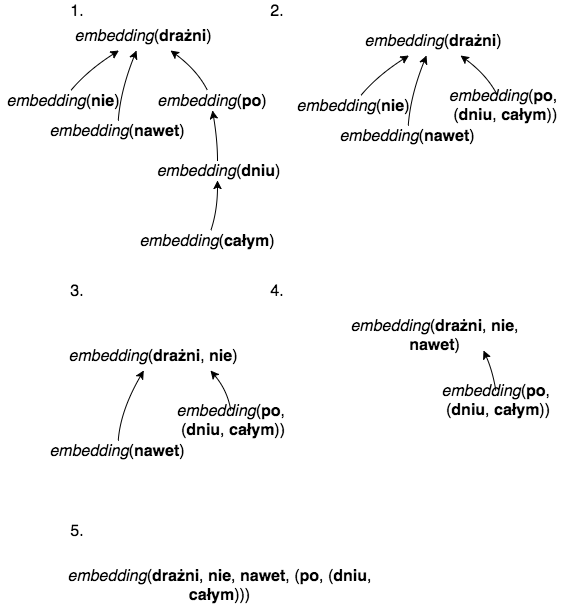
\includegraphics[width=0.5\textwidth]{imgs/niedrazniex}
		\caption{An example of combining dependent phrases with their parent in the Sequential Child-Combination Tree-LSTM model.}
		\label{tab:niedrazniex}
	\end{center}
\end{figure}
	
\section{Evaluation} 
	The model proposed in this paper was evaluated on the held-out test set provided in the PolEval 2017 competition. As baselines, we used a simple, linearly chained LSTM network, Conditional Random Fields \cite{lafferty2001conditional} with rather standard contextual and word-shape features and no syntactic information as well as the Child-Sum Tree LSTM model mentioned above. The result submitted to the single-blind evaluation stage of the PolEval competition was approx. 76,80\% accuracy of sentiment label assignments. In Table \ref{tab:evaluation} we report the best results obtained on the same test set with a modification of our originally submitted system, which involved lemmatizing the word tokens in the training and test sentences. After this modification, our approach seems to have slightly outperformed the Child-Sum Tree model on the PolEval test set. It is interesting to note that some improvement resulting from lemmatization was consistent across the different approaches we tested.
\begin{table}[h]
 \begin{center}
\begin{tabular}{|l|l|}

      \hline
      %Level&Tools\\
      %\hline\hline
      Model & Score\\
      \hline
      \hline
      LSTM &70,70\%\\
      \hline
      Lemmatized CRF & 75,63\%\\
      \hline
      Child-Sum Tree-LSTM &  77,69\%\\
      \hline
      Sequential Child-Combination & \\
      Tree-LSTM & \textbf{76,80}\%\\
      \hline
      Lemmatized Child-Sum Tree-LSTM & 79,35\%\\
      \hline
      Lemmatized Sequential Child-Combination & \\
      Tree-LSTM & \textbf{79,89\%} \\
      \hline
\end{tabular}
\caption{Sentiment classification accuracy on the PolEval test set.}
\label{tab:evaluation}
 \end{center}
\end{table}



\section{Conclusions and future work}

In the present paper we described a Sequential Child-Combination Tree-LSTM model for the task of syntax-based sentiment analysis in Polish. The theoretical motivation behind this model was to provide a relatively robust mechanism of considering syntactic relations between words and phrases in natural language sentences as a potentially relevant feature in sentiment detection. In particular, we proposed a mechanism of compositionally generating governor or parent-phrase embeddings from the embeddings of their dependent phrases, which preserves some of the compositionality of the latter type of units. The results obtained for the PolEval 2017 test set were promising, but given the rather limited size of these datasets, it would be necessary to run similar comparisons on larger sentiment treebanks, in order to validate the proposed approach of tracking the syntactic and semantic compositionality of sentences in SA. The method described in this paper can be applied to dependency-parsed data in other languages, possibly also in other tasks, such as measuring the semantic relatedness of sentence pairs, where syntax-driven deep learning approaches proved to be particularly successful \cite{tai2015improved}.
\section{Availability}

The source code of the system described in this paper, together with its trained models are available at \url{https://github.com/michal-lew/tree-lstm}.

%\nocite{*}

\section{Acknowledgments}

Research described in this paper was carried out within a grant funded
by the European Union Regional Operation Program for
the Pomeranian Voivodship for the years 2014-2020 based on
the Resolution no 190/214/17 of the Pomeranian Voivodship
Board, project RPPM.01.01.01-22-0026/16.

\bibliographystyle{ltc05}
\bibliography{sal} 

\end{document}

